\documentclass[11pt]{article}
\usepackage[textwidth=18.0cm, textheight=23.0cm, top=2.0cm]{geometry}
\usepackage{pst-all}
\usepackage{amssymb}
\usepackage{tikz}
\usepackage{underscore}\begin{document}
\pagestyle{empty}


ClassName: \underline{\textbf{Class_10.2bp-15}}
\par
BinSize: \underline{\textbf{100 × 100}}
\par
ReduceSize: \underline{\textbf{100 × 100}}
\par
TypeNum: \underline{\textbf{40}}
\par
Num: \underline{\textbf{40}}
\par
OutS: \underline{\textbf{60000}}
\par
InS: \underline{\textbf{49619}}
\par
Rate: \underline{\textbf{0.827}}
\par
UB: \underline{\textbf{6}}
\par
LB0: \underline{\textbf{6}}
\par
LB: \underline{\textbf{6}}
\par
LBWithCut: \underline{\textbf{6}}
\par
NodeCut: \underline{\textbf{0}}
\par
ExtendedNodeCnt: \underline{\textbf{1}}
\par
GenNodeCnt: \underline{\textbf{1}}
\par
PrimalNode: \underline{\textbf{0}}
\par
ColumnCount: \underline{\textbf{6}}
\par
TotalCutCount: \underline{\textbf{0}}
\par
RootCutCount: \underline{\textbf{0}}
\par
LPSolverCnt: \underline{\textbf{1}}
\par
PricingSolverCnt: \underline{\textbf{0}}
\par
BranchAndBoundNum: \underline{\textbf{1}}
\par
isOpt: \underline{\textbf{true}}
\par
TimeOnInitSolution: \underline{\textbf{600.000 s}}
\par
TimeOnPrimal: \underline{\textbf{0.000 s}}
\par
TimeOnPricing: \underline{\textbf{0.000 s}}
\par
TimeOnRmp: \underline{\textbf{0.062 s}}
\par
TotalTime: \underline{\textbf{600.312 s}}
\par
\newpage


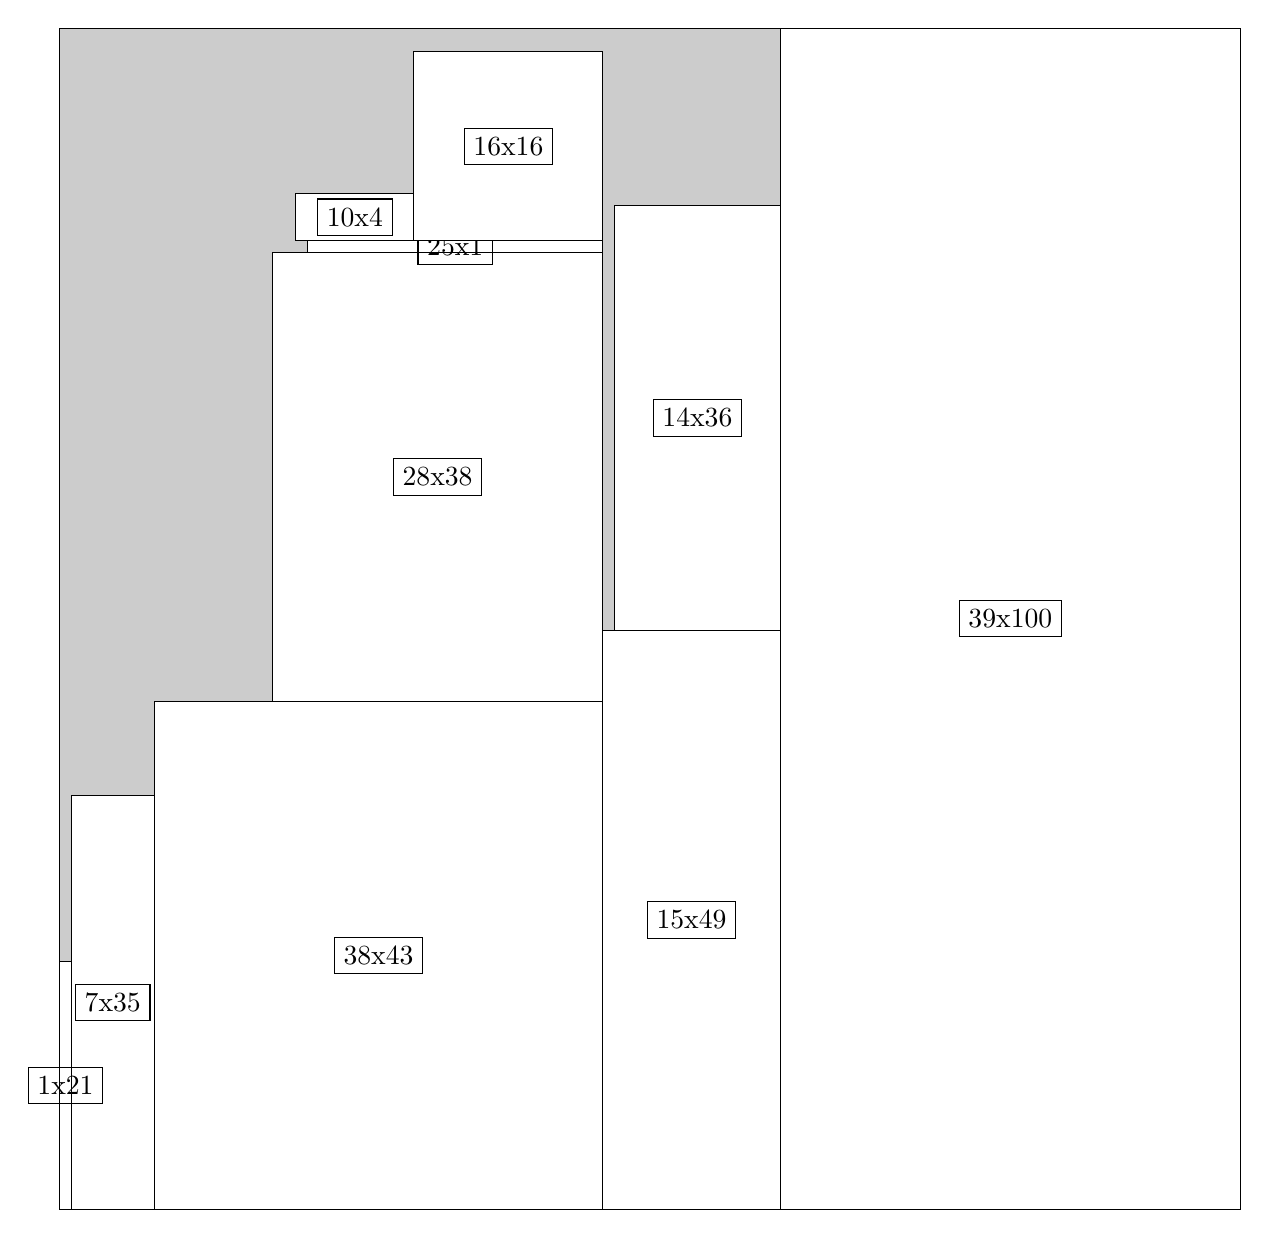
\begin{tikzpicture}[shorten >=1pt,scale=1.0,every node/.style={scale=1.0},->]
\tikzstyle{vertex}=[circle,fill=black!25,minimum size=14pt,inner sep=0pt]
\filldraw[fill=gray!40!white, draw=black] (0,0) rectangle (15.0,15.0);
\foreach \name/\x/\y/\w/\h in {39x100/9.15/0.0/5.85/15.0,15x49/6.8999999999999995/0.0/2.25/7.35,14x36/7.05/7.35/2.1/5.3999999999999995,38x43/1.2/0.0/5.7/6.45,28x38/2.6999999999999997/6.45/4.2/5.7,25x1/3.15/12.15/3.75/0.15,16x16/4.5/12.299999999999999/2.4/2.4,10x4/3.0/12.299999999999999/1.5/0.6,7x35/0.15/0.0/1.05/5.25,1x21/0.0/0.0/0.15/3.15}
\filldraw[fill=white!40!white, draw=black] (\x,\y) rectangle node[draw] (\name) {\name} ++(\w,\h);
\end{tikzpicture}


w =39 , h =100 , x =61 , y =0 , v =3900
\par
w =15 , h =49 , x =46 , y =0 , v =735
\par
w =14 , h =36 , x =47 , y =49 , v =504
\par
w =38 , h =43 , x =8 , y =0 , v =1634
\par
w =28 , h =38 , x =18 , y =43 , v =1064
\par
w =25 , h =1 , x =21 , y =81 , v =25
\par
w =16 , h =16 , x =30 , y =82 , v =256
\par
w =10 , h =4 , x =20 , y =82 , v =40
\par
w =7 , h =35 , x =1 , y =0 , v =245
\par
w =1 , h =21 , x =0 , y =0 , v =21
\par
\newpage


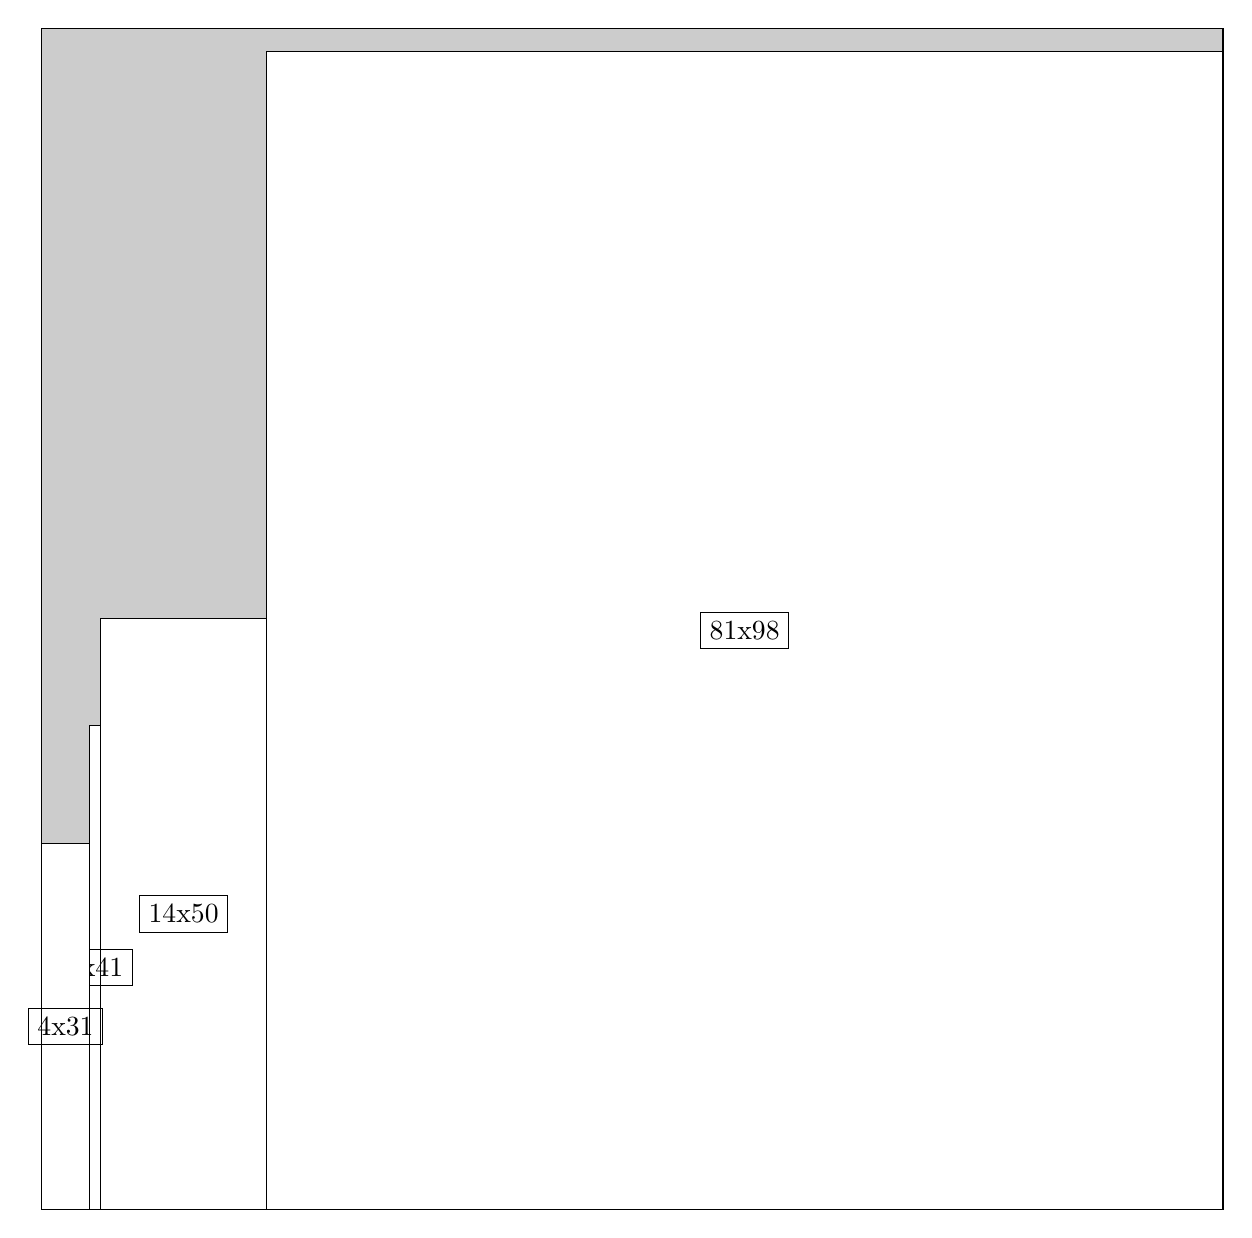
\begin{tikzpicture}[shorten >=1pt,scale=1.0,every node/.style={scale=1.0},->]
\tikzstyle{vertex}=[circle,fill=black!25,minimum size=14pt,inner sep=0pt]
\filldraw[fill=gray!40!white, draw=black] (0,0) rectangle (15.0,15.0);
\foreach \name/\x/\y/\w/\h in {81x98/2.85/0.0/12.15/14.7,14x50/0.75/0.0/2.1/7.5,1x41/0.6/0.0/0.15/6.1499999999999995,4x31/0.0/0.0/0.6/4.6499999999999995}
\filldraw[fill=white!40!white, draw=black] (\x,\y) rectangle node[draw] (\name) {\name} ++(\w,\h);
\end{tikzpicture}


w =81 , h =98 , x =19 , y =0 , v =7938
\par
w =14 , h =50 , x =5 , y =0 , v =700
\par
w =1 , h =41 , x =4 , y =0 , v =41
\par
w =4 , h =31 , x =0 , y =0 , v =124
\par
\newpage


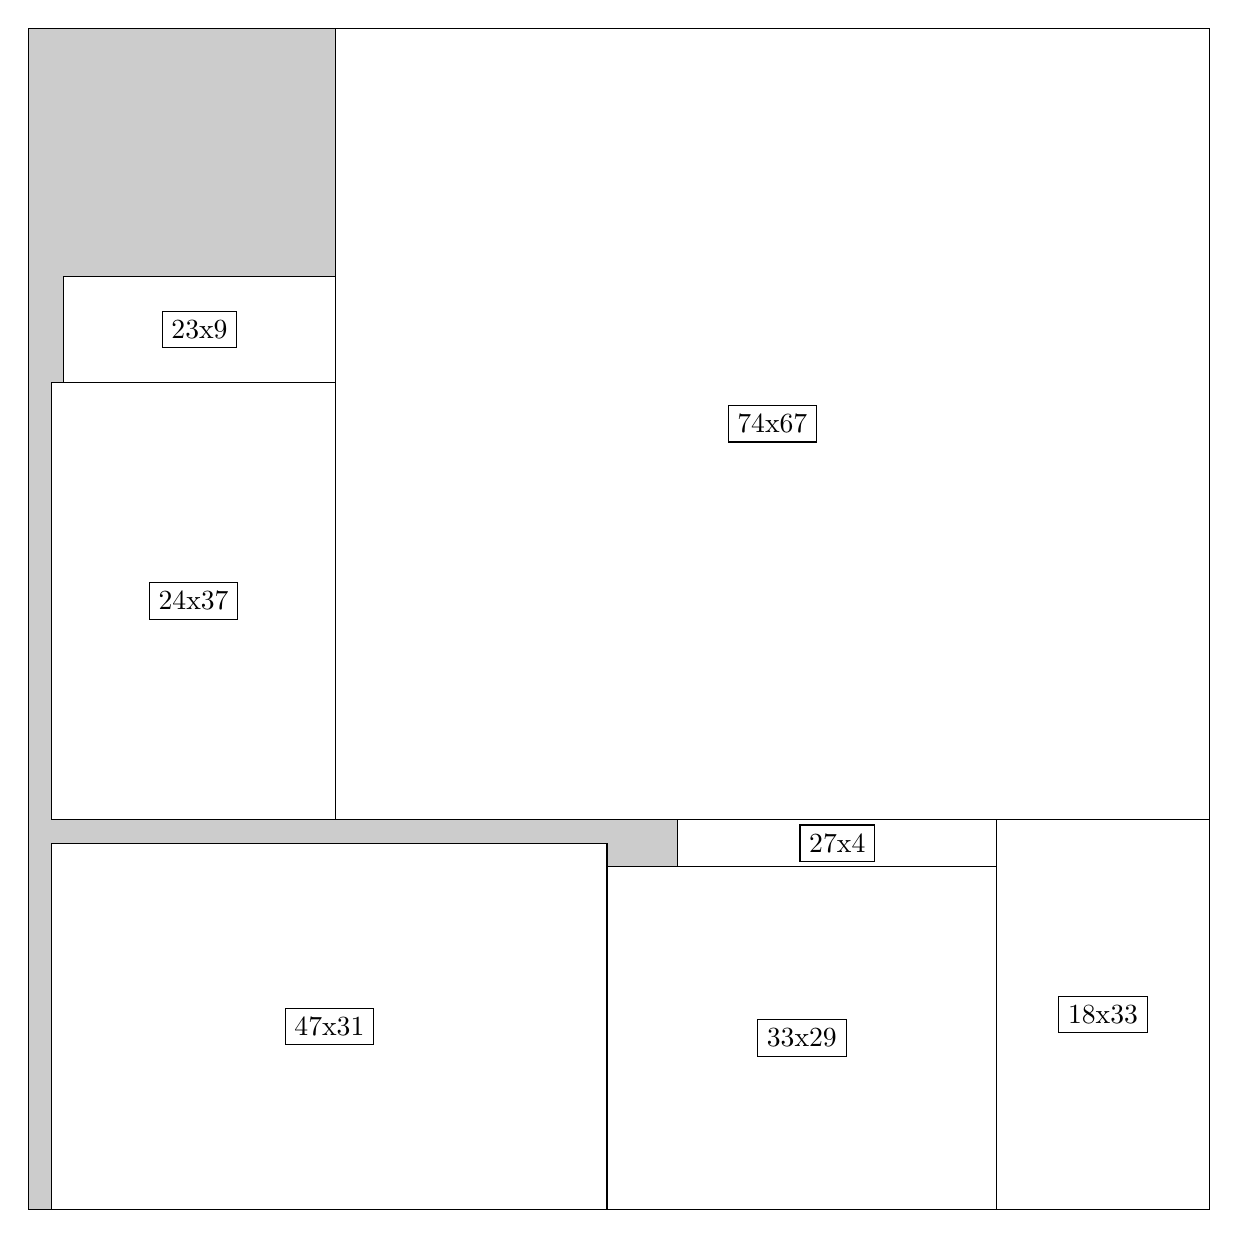
\begin{tikzpicture}[shorten >=1pt,scale=1.0,every node/.style={scale=1.0},->]
\tikzstyle{vertex}=[circle,fill=black!25,minimum size=14pt,inner sep=0pt]
\filldraw[fill=gray!40!white, draw=black] (0,0) rectangle (15.0,15.0);
\foreach \name/\x/\y/\w/\h in {18x33/12.299999999999999/0.0/2.6999999999999997/4.95,33x29/7.35/0.0/4.95/4.35,27x4/8.25/4.35/4.05/0.6,47x31/0.3/0.0/7.05/4.6499999999999995,74x67/3.9/4.95/11.1/10.049999999999999,24x37/0.3/4.95/3.5999999999999996/5.55,23x9/0.44999999999999996/10.5/3.4499999999999997/1.3499999999999999}
\filldraw[fill=white!40!white, draw=black] (\x,\y) rectangle node[draw] (\name) {\name} ++(\w,\h);
\end{tikzpicture}


w =18 , h =33 , x =82 , y =0 , v =594
\par
w =33 , h =29 , x =49 , y =0 , v =957
\par
w =27 , h =4 , x =55 , y =29 , v =108
\par
w =47 , h =31 , x =2 , y =0 , v =1457
\par
w =74 , h =67 , x =26 , y =33 , v =4958
\par
w =24 , h =37 , x =2 , y =33 , v =888
\par
w =23 , h =9 , x =3 , y =70 , v =207
\par
\newpage


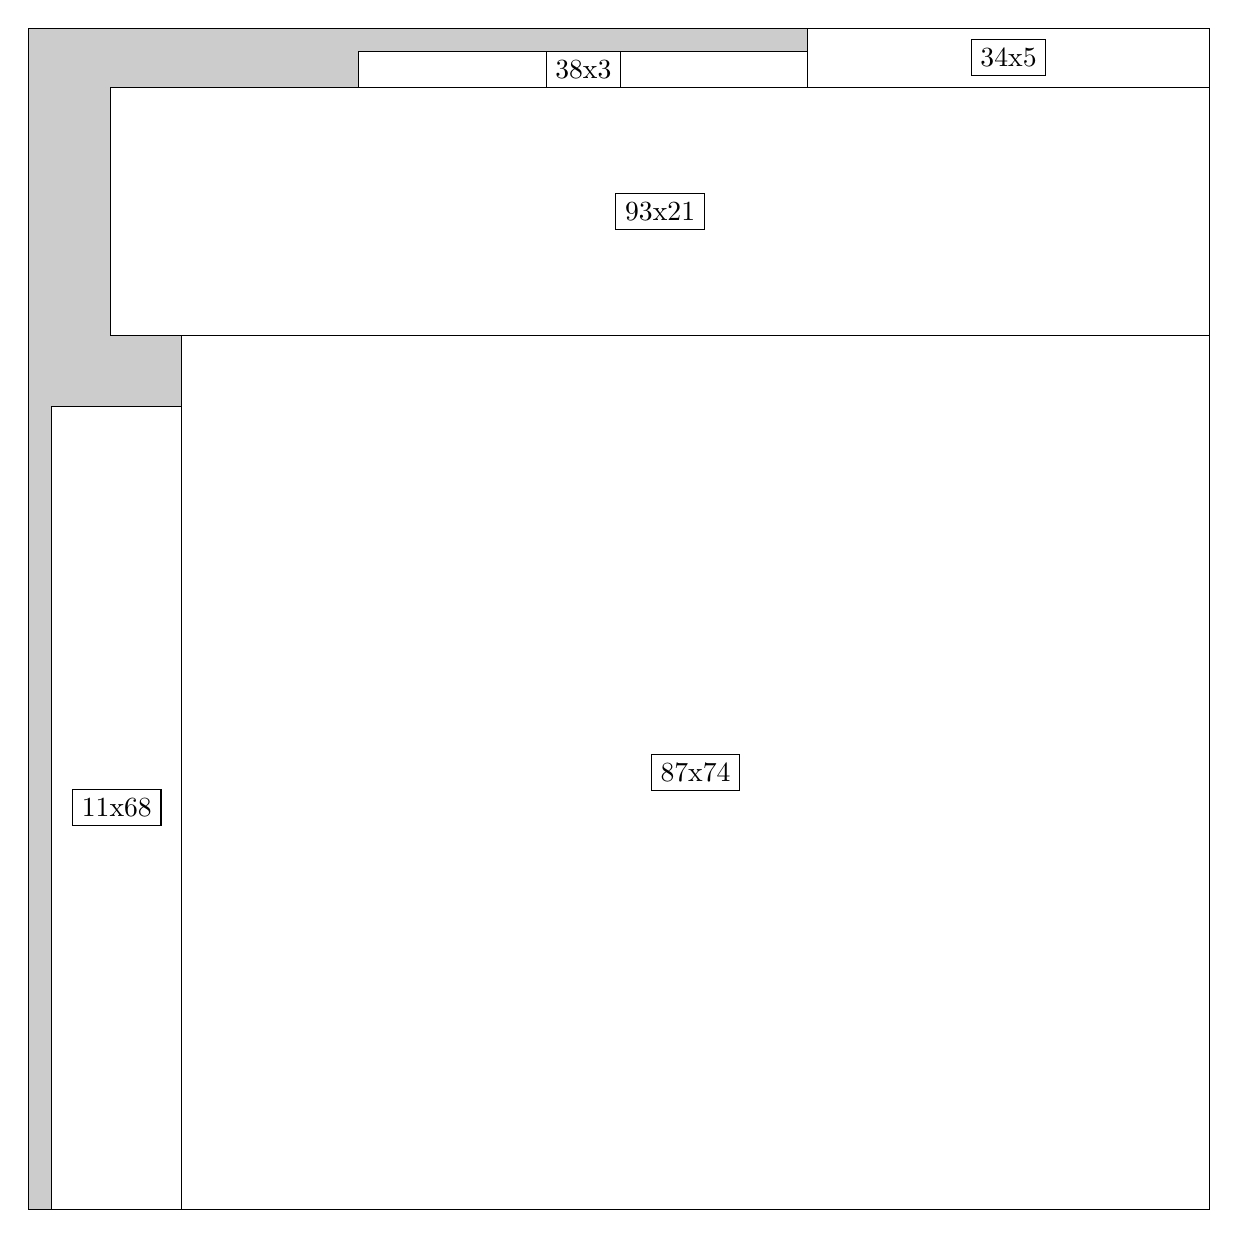
\begin{tikzpicture}[shorten >=1pt,scale=1.0,every node/.style={scale=1.0},->]
\tikzstyle{vertex}=[circle,fill=black!25,minimum size=14pt,inner sep=0pt]
\filldraw[fill=gray!40!white, draw=black] (0,0) rectangle (15.0,15.0);
\foreach \name/\x/\y/\w/\h in {87x74/1.95/0.0/13.049999999999999/11.1,11x68/0.3/0.0/1.65/10.2,93x21/1.05/11.1/13.95/3.15,34x5/9.9/14.25/5.1/0.75,38x3/4.2/14.25/5.7/0.44999999999999996}
\filldraw[fill=white!40!white, draw=black] (\x,\y) rectangle node[draw] (\name) {\name} ++(\w,\h);
\end{tikzpicture}


w =87 , h =74 , x =13 , y =0 , v =6438
\par
w =11 , h =68 , x =2 , y =0 , v =748
\par
w =93 , h =21 , x =7 , y =74 , v =1953
\par
w =34 , h =5 , x =66 , y =95 , v =170
\par
w =38 , h =3 , x =28 , y =95 , v =114
\par
\newpage


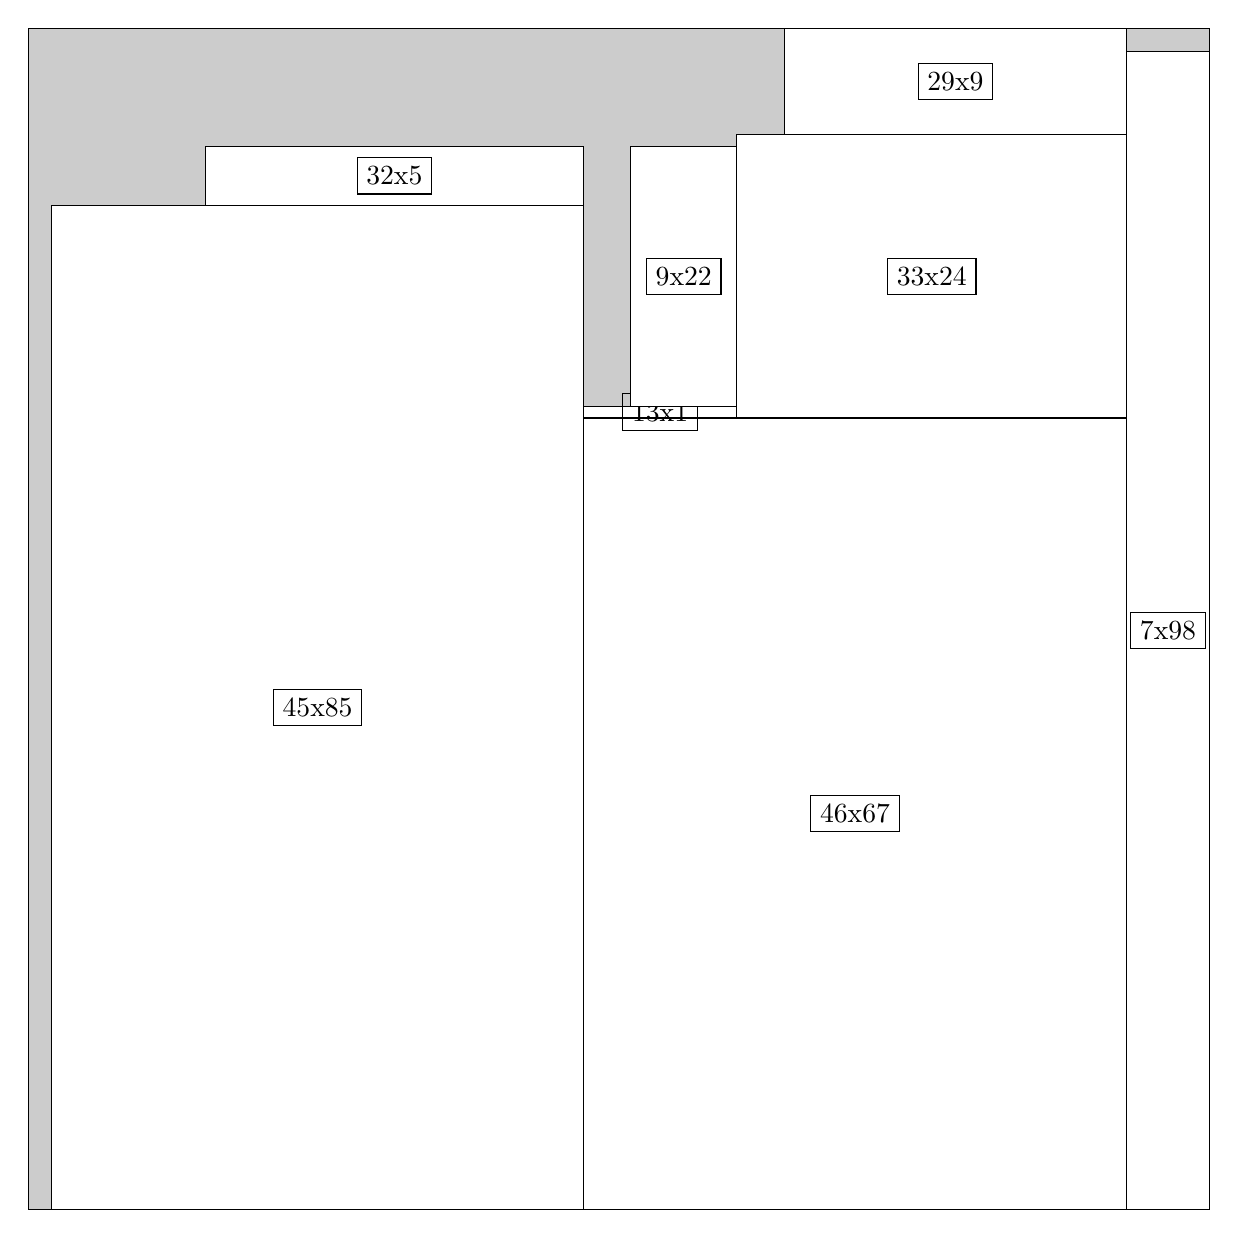
\begin{tikzpicture}[shorten >=1pt,scale=1.0,every node/.style={scale=1.0},->]
\tikzstyle{vertex}=[circle,fill=black!25,minimum size=14pt,inner sep=0pt]
\filldraw[fill=gray!40!white, draw=black] (0,0) rectangle (15.0,15.0);
\foreach \name/\x/\y/\w/\h in {7x98/13.95/0.0/1.05/14.7,46x67/7.05/0.0/6.8999999999999995/10.049999999999999,33x24/9.0/10.049999999999999/4.95/3.5999999999999996,13x1/7.05/10.049999999999999/1.95/0.15,9x22/7.6499999999999995/10.2/1.3499999999999999/3.3,29x9/9.6/13.65/4.35/1.3499999999999999,45x85/0.3/0.0/6.75/12.75,32x5/2.25/12.75/4.8/0.75}
\filldraw[fill=white!40!white, draw=black] (\x,\y) rectangle node[draw] (\name) {\name} ++(\w,\h);
\end{tikzpicture}


w =7 , h =98 , x =93 , y =0 , v =686
\par
w =46 , h =67 , x =47 , y =0 , v =3082
\par
w =33 , h =24 , x =60 , y =67 , v =792
\par
w =13 , h =1 , x =47 , y =67 , v =13
\par
w =9 , h =22 , x =51 , y =68 , v =198
\par
w =29 , h =9 , x =64 , y =91 , v =261
\par
w =45 , h =85 , x =2 , y =0 , v =3825
\par
w =32 , h =5 , x =15 , y =85 , v =160
\par
\newpage


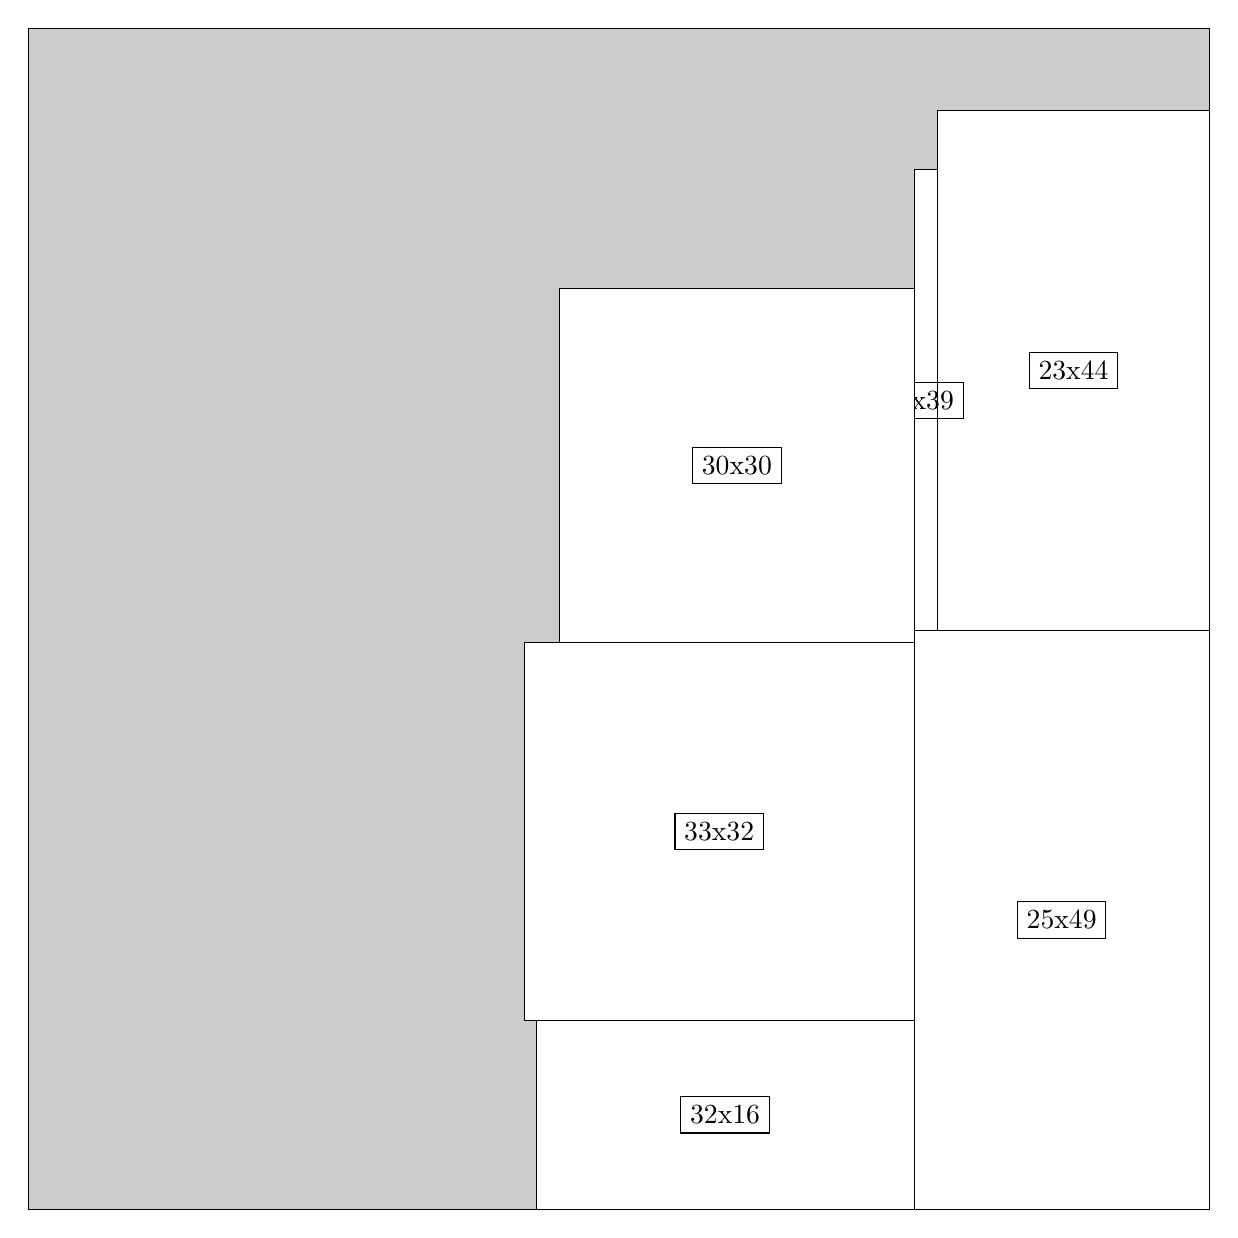
\begin{tikzpicture}[shorten >=1pt,scale=1.0,every node/.style={scale=1.0},->]
\tikzstyle{vertex}=[circle,fill=black!25,minimum size=14pt,inner sep=0pt]
\filldraw[fill=gray!40!white, draw=black] (0,0) rectangle (15.0,15.0);
\foreach \name/\x/\y/\w/\h in {25x49/11.25/0.0/3.75/7.35,23x44/11.549999999999999/7.35/3.4499999999999997/6.6,2x39/11.25/7.35/0.3/5.85,32x16/6.45/0.0/4.8/2.4,33x32/6.3/2.4/4.95/4.8,30x30/6.75/7.199999999999999/4.5/4.5}
\filldraw[fill=white!40!white, draw=black] (\x,\y) rectangle node[draw] (\name) {\name} ++(\w,\h);
\end{tikzpicture}


w =25 , h =49 , x =75 , y =0 , v =1225
\par
w =23 , h =44 , x =77 , y =49 , v =1012
\par
w =2 , h =39 , x =75 , y =49 , v =78
\par
w =32 , h =16 , x =43 , y =0 , v =512
\par
w =33 , h =32 , x =42 , y =16 , v =1056
\par
w =30 , h =30 , x =45 , y =48 , v =900
\par
\newpage


\end{document}